%% This is an example first chapter.  You should put chapter/appendix that you
%% write into a separate file, and add a line \include{yourfilename} to
%% main.tex, where `yourfilename.tex' is the name of the chapter/appendix file.
%% You can process specific files by typing their names in at the 
%% \files=
%% prompt when you run the file main.tex through LaTeX.
\chapter{Experiments}
\label{chap:experiments}

% % remove all spaces between columns in tables
% \setlength{\tabcolsep}{0.3pt}
% % remove all spaces below captions
% \setlength{\belowcaptionskip}{-5pt}

In this chapter, we first introduce our synthetic dataset, this dataset contains IMU measurements and corresponding visual frames, it also provides the ground truth IMU-camera pose to be used in evaluation stage. We then perform some experiments to show that our visual-inertial odometry has good accuracy and low computational cost in several different experimental settings.

\section{Synthetic Dataset}
\label{sec:sync_data}

\begin{table}[t]
\centering
\begin{tabular}{|c || P{2.5cm} | P{2.5cm} | P{6.5cm}|} 
\hline
 Name & Overall Duration $\left[ s \right]$ & Travelled Distance $\left[ m \right]$ & Description \\
 \hline
 001 & 10.0 & TODO & Pure movement without rotation \\ 
 002 & 10.0 & 0.0 & Pure rotation without translation \\ 
 003 & 30.0 & 118.99 & Random straight trajectory \\ 
 004 & 120.0 & 257.71 & Random circle-like trajectory \\ 
 \hline
\end{tabular}
     \caption{Trajectories we create for experiments, the datasets are named after the corresponding trajectories. Noted that \textbf{001} and \textbf{002} are ideal trajectories to test the correctness and performance of ESKF IMU integration. The trajectory \textbf{003} and \textbf{004} try to simulate the trajectories of micro helicopter by setting the similar velocity and pose.}
    \label{table:tb1}
\end{table}

\begin{figure}
\centering
	\begin{subfloat}[Trajectory 003]{
		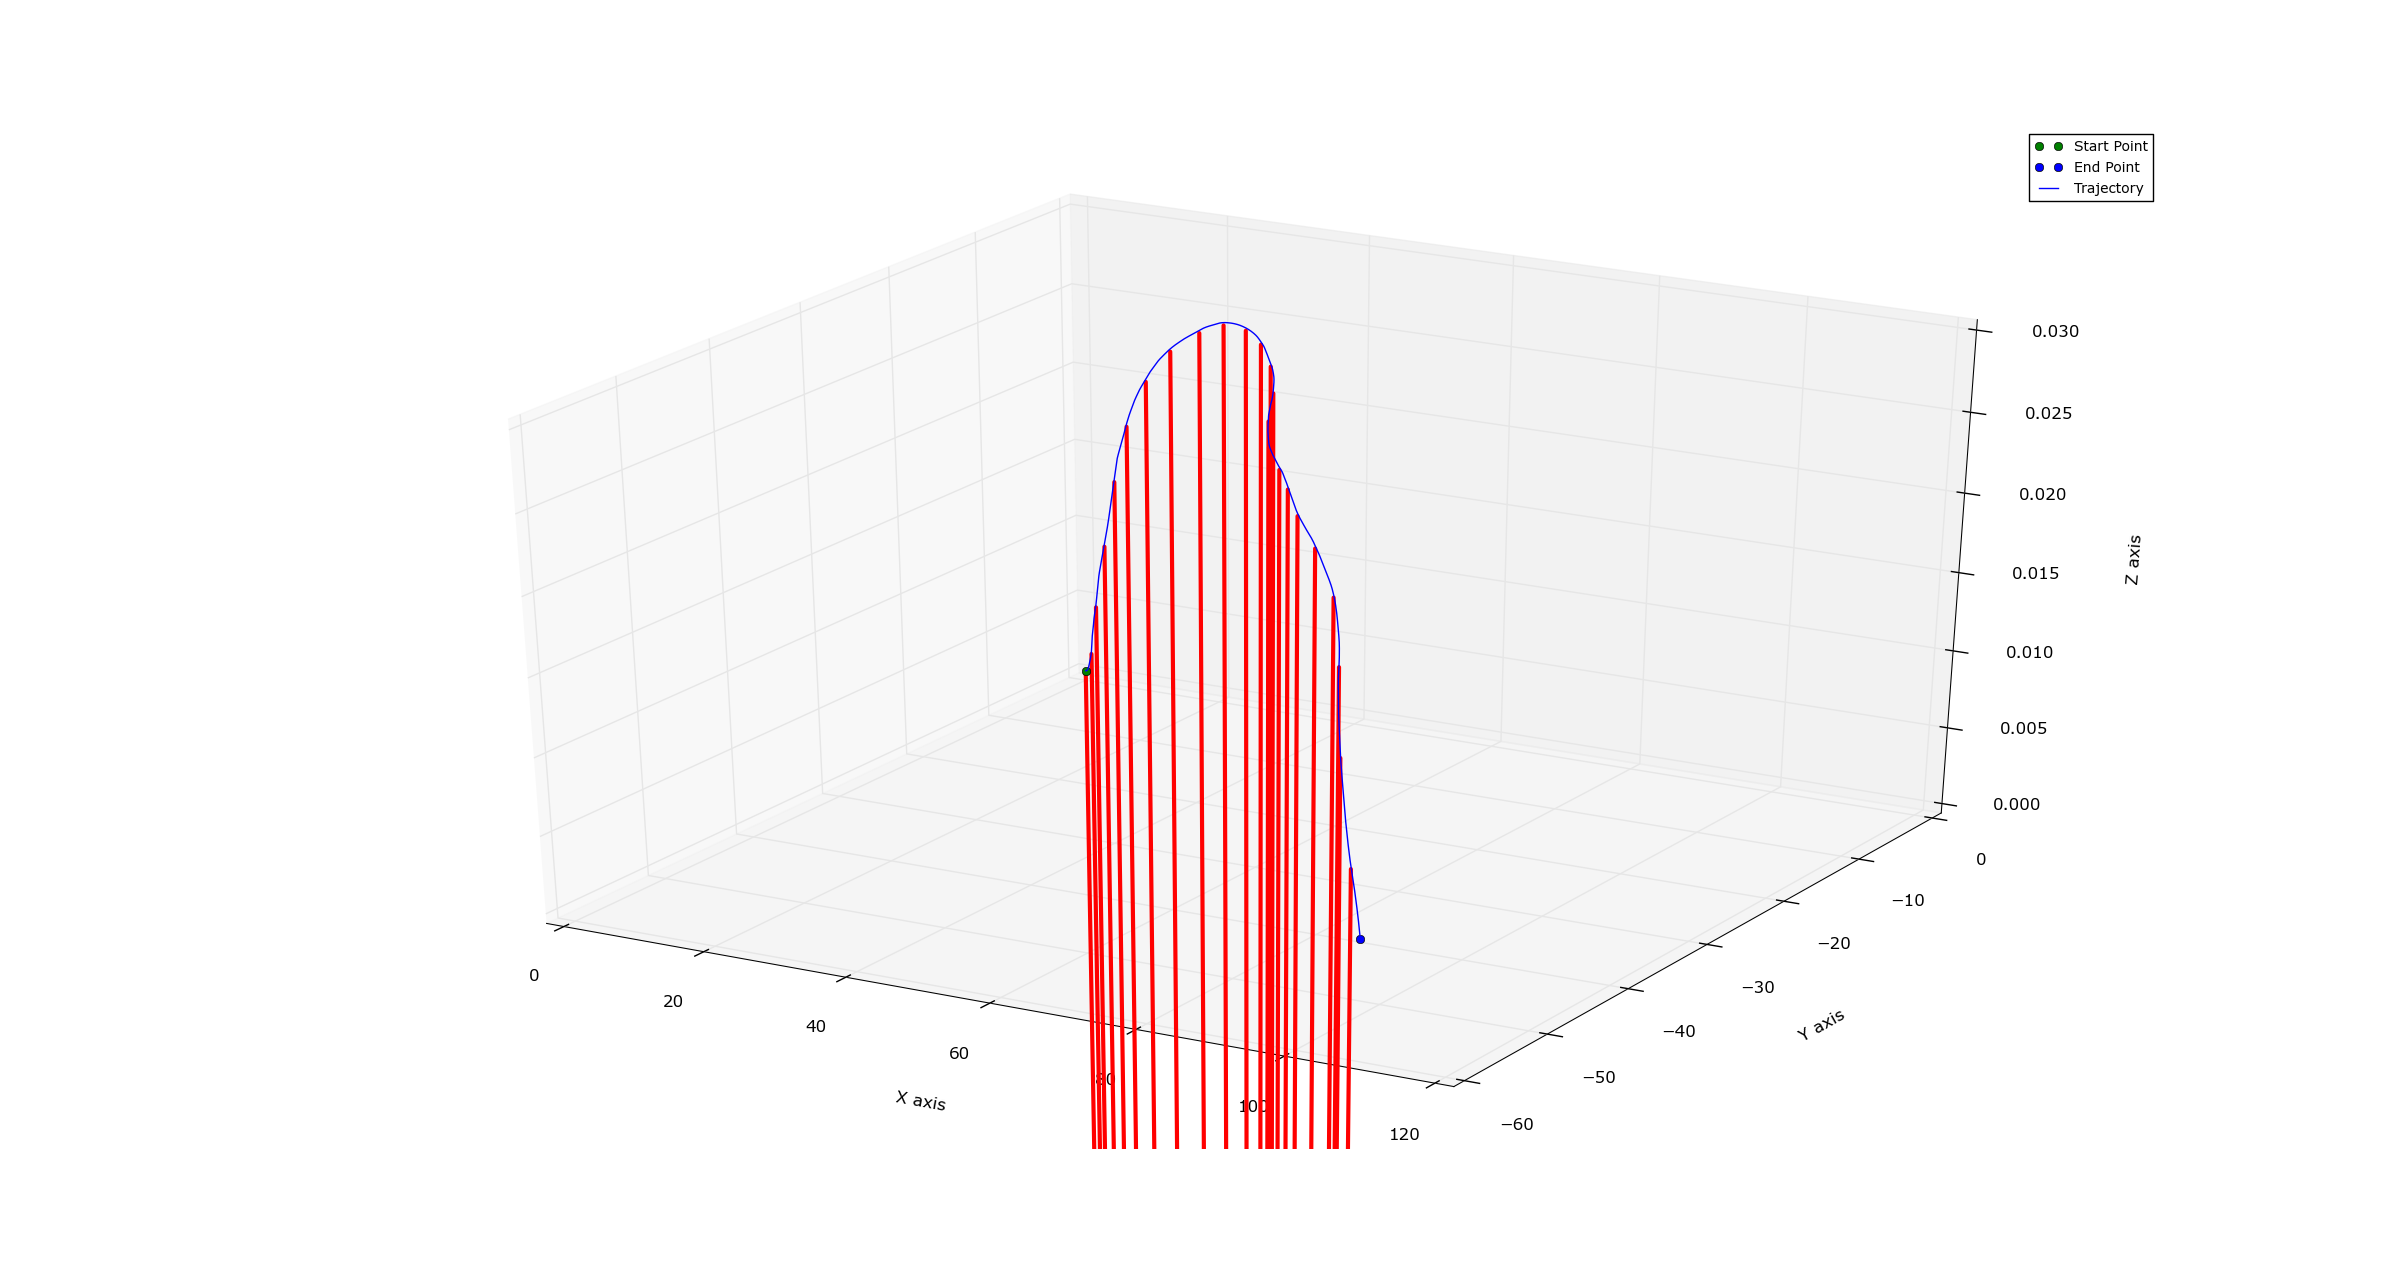
\includegraphics[width=0.4\textwidth]{CONTENT/Figure/Figure5-1a.png}
		\label{fig:fig5-1-a}}
	\end{subfloat}\qquad
	\begin{subfloat}[Trajectory 004]{
		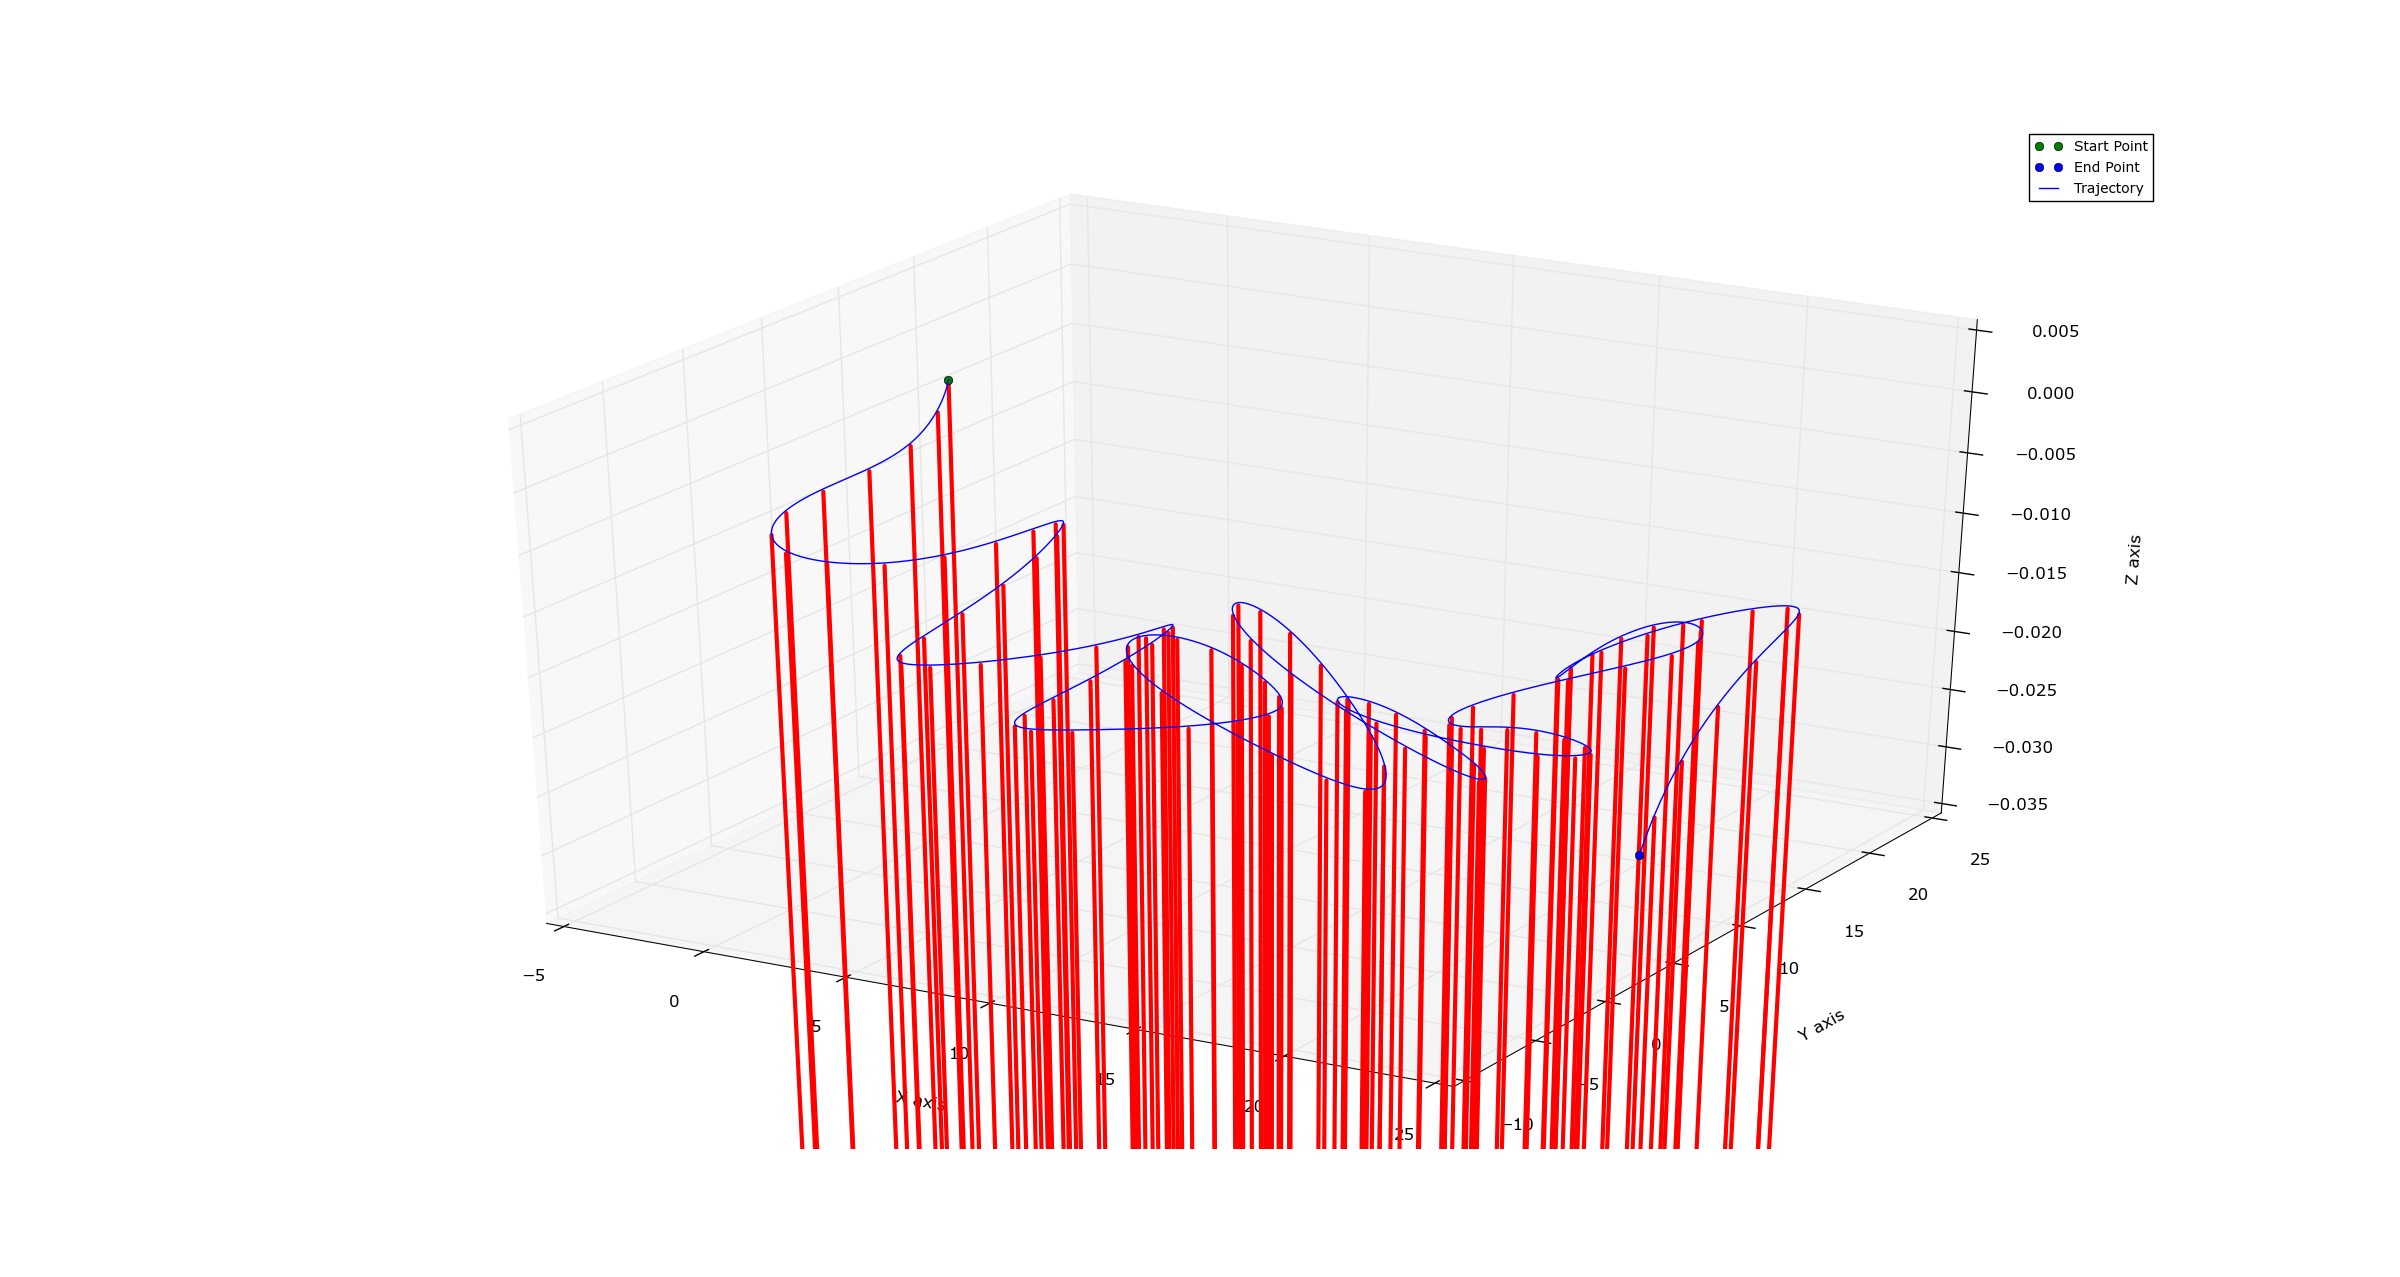
\includegraphics[width=0.4\textwidth]{CONTENT/Figure/Figure5-1b.png}
		\label{fig:fig5-1-b}}
	\end{subfloat}
	
	%\hspace*{\fill} % separation between the subfigures
	
	\caption{Visualization of trajectory \textbf{003} and trajectory \textbf{004}. } 
	\label{fig:fig5-1}
\end{figure}

We use a synthetic IMU-camera dataset in this master thesis because it has following advantages rather than real dataset
\begin{itemize}
\item {Noises in synthetic dataset is controllable. Though we have considered the noise model in our work, the types of noises in real data varies. Besides, denoising from such as IMU sensor is beyond the content of this master thesis. }
\item {Synchronization between IMU and camera is annoying. Though we know the frequency of camera and IMU from datasheet or introduction, the real output might still differ, \eg, the first image frame might correspond to fourth IMU measurement in first trial but changes to fifth IMU measurement in next trial. In synthetic data, we could use aligned IMU and camera data.}
\item {Synthetic data is more flexible. We could generate the special trajectory, \ie, a pure rotation sequence. However it is hard to create such a sequence in real platform.}
\item {Synthetic data can provide accurate ground truth data at each timestamp. In real platform, a evaluation of position drift usually only happens at end point, \eg, setting the start point as same as end point and measure the drift. Motion capture system can provide ground truth data at each timestamp, however accuracy of such system usually is not high as synthetic data.}
\item {Numerous calibration steps are saved. In real equipment, it is normal to calibrate the device again after several uses. We can ignore the calibration process in simulated platforms.}
\end{itemize}
Also to best of our knowledge, there is no open sourced IMU-camera synthetic data set, hence we decide to generate our own IMU-camera synthetic dataset.

\

\textbf{Trajectory} We start to generate synthetic data by first defining the trajectory of our IMU-camera platform. As we explain before, we assume the camera and IMU sensor share an identical pose in all our experiments for simplification. We have created four different types of trajectory showed in Table \ref{table:tb1}. Dataset \textbf{001} and Dataset \textbf{002} is used to evaluate the performance of ESKF IMU integration as we use ground-truth data in \textit{correction step}; And Dataset \textbf{003} and Dataset \textbf{004} test the performance of visual-inertial odometry which \textbf{004} has longer travelled distance. We have made following several general assumptions of trajectories,
\begin{itemize}
\item{We assume the initial position of trajectory as $(0, 0, 0)$ in global frame, and initial orientation as quaternion $(1, 0, 0, 0)$ which points at the positive z axis of global coordinate system.}
\item{We assume the second derivative of position and orientation remains constant within two successive sensor samplings.}
\item{We assume the second derivative of position and orientation obeys a normal distribution with additional white Gaussian noise.}
\end{itemize}
we illustrate trajectory \textbf{003} and \textbf{004} in Figure \ref{fig:fig5-1}.

\

\textbf{Synthetic IMU data} We then use IMUSim \cite{young2011imusim} to simulate IMU data by our customized trajectory. IMUSim is a powerful python-based open-sourced IMU simulation tool, which models a wide range of real-world environments and/or external noises. To obtain more realistic IMU data, we set the output frequency of IMU as 100 [Hz], sensitivity of gyroscope is 1200 [deg/s] and sensitivity of accelerometer is 4 gravity. The whole IMU model is noise-free with some additional white Gaussian noise. Overall we have 3-vector gyroscope readings, 3-vector accelerometer readings, 3-vector ground truth position, 4-vector ground truth orientation from IMUSim for single IMU sampling.

\

\textbf{Synthetic visual data} Blender \cite{wiki:blender} is the main tool that creates virtual scene for our experiments. 

\section{Some other experiments}